\chapter{Bijlages}
\label{ch:bijlages}

Om de leesbaarheid van de bachelorproef te behouden zijn sommige niet essentiële afbeeldingen, tabellen en overige documenten in dit hoofdstuk opgenomen. 

\section{Screenshots afbeeldingsevaluatietool}
\label{sec:bijlages-screenshot-afbeeldingsevaluatietool}

\begin{figure}
	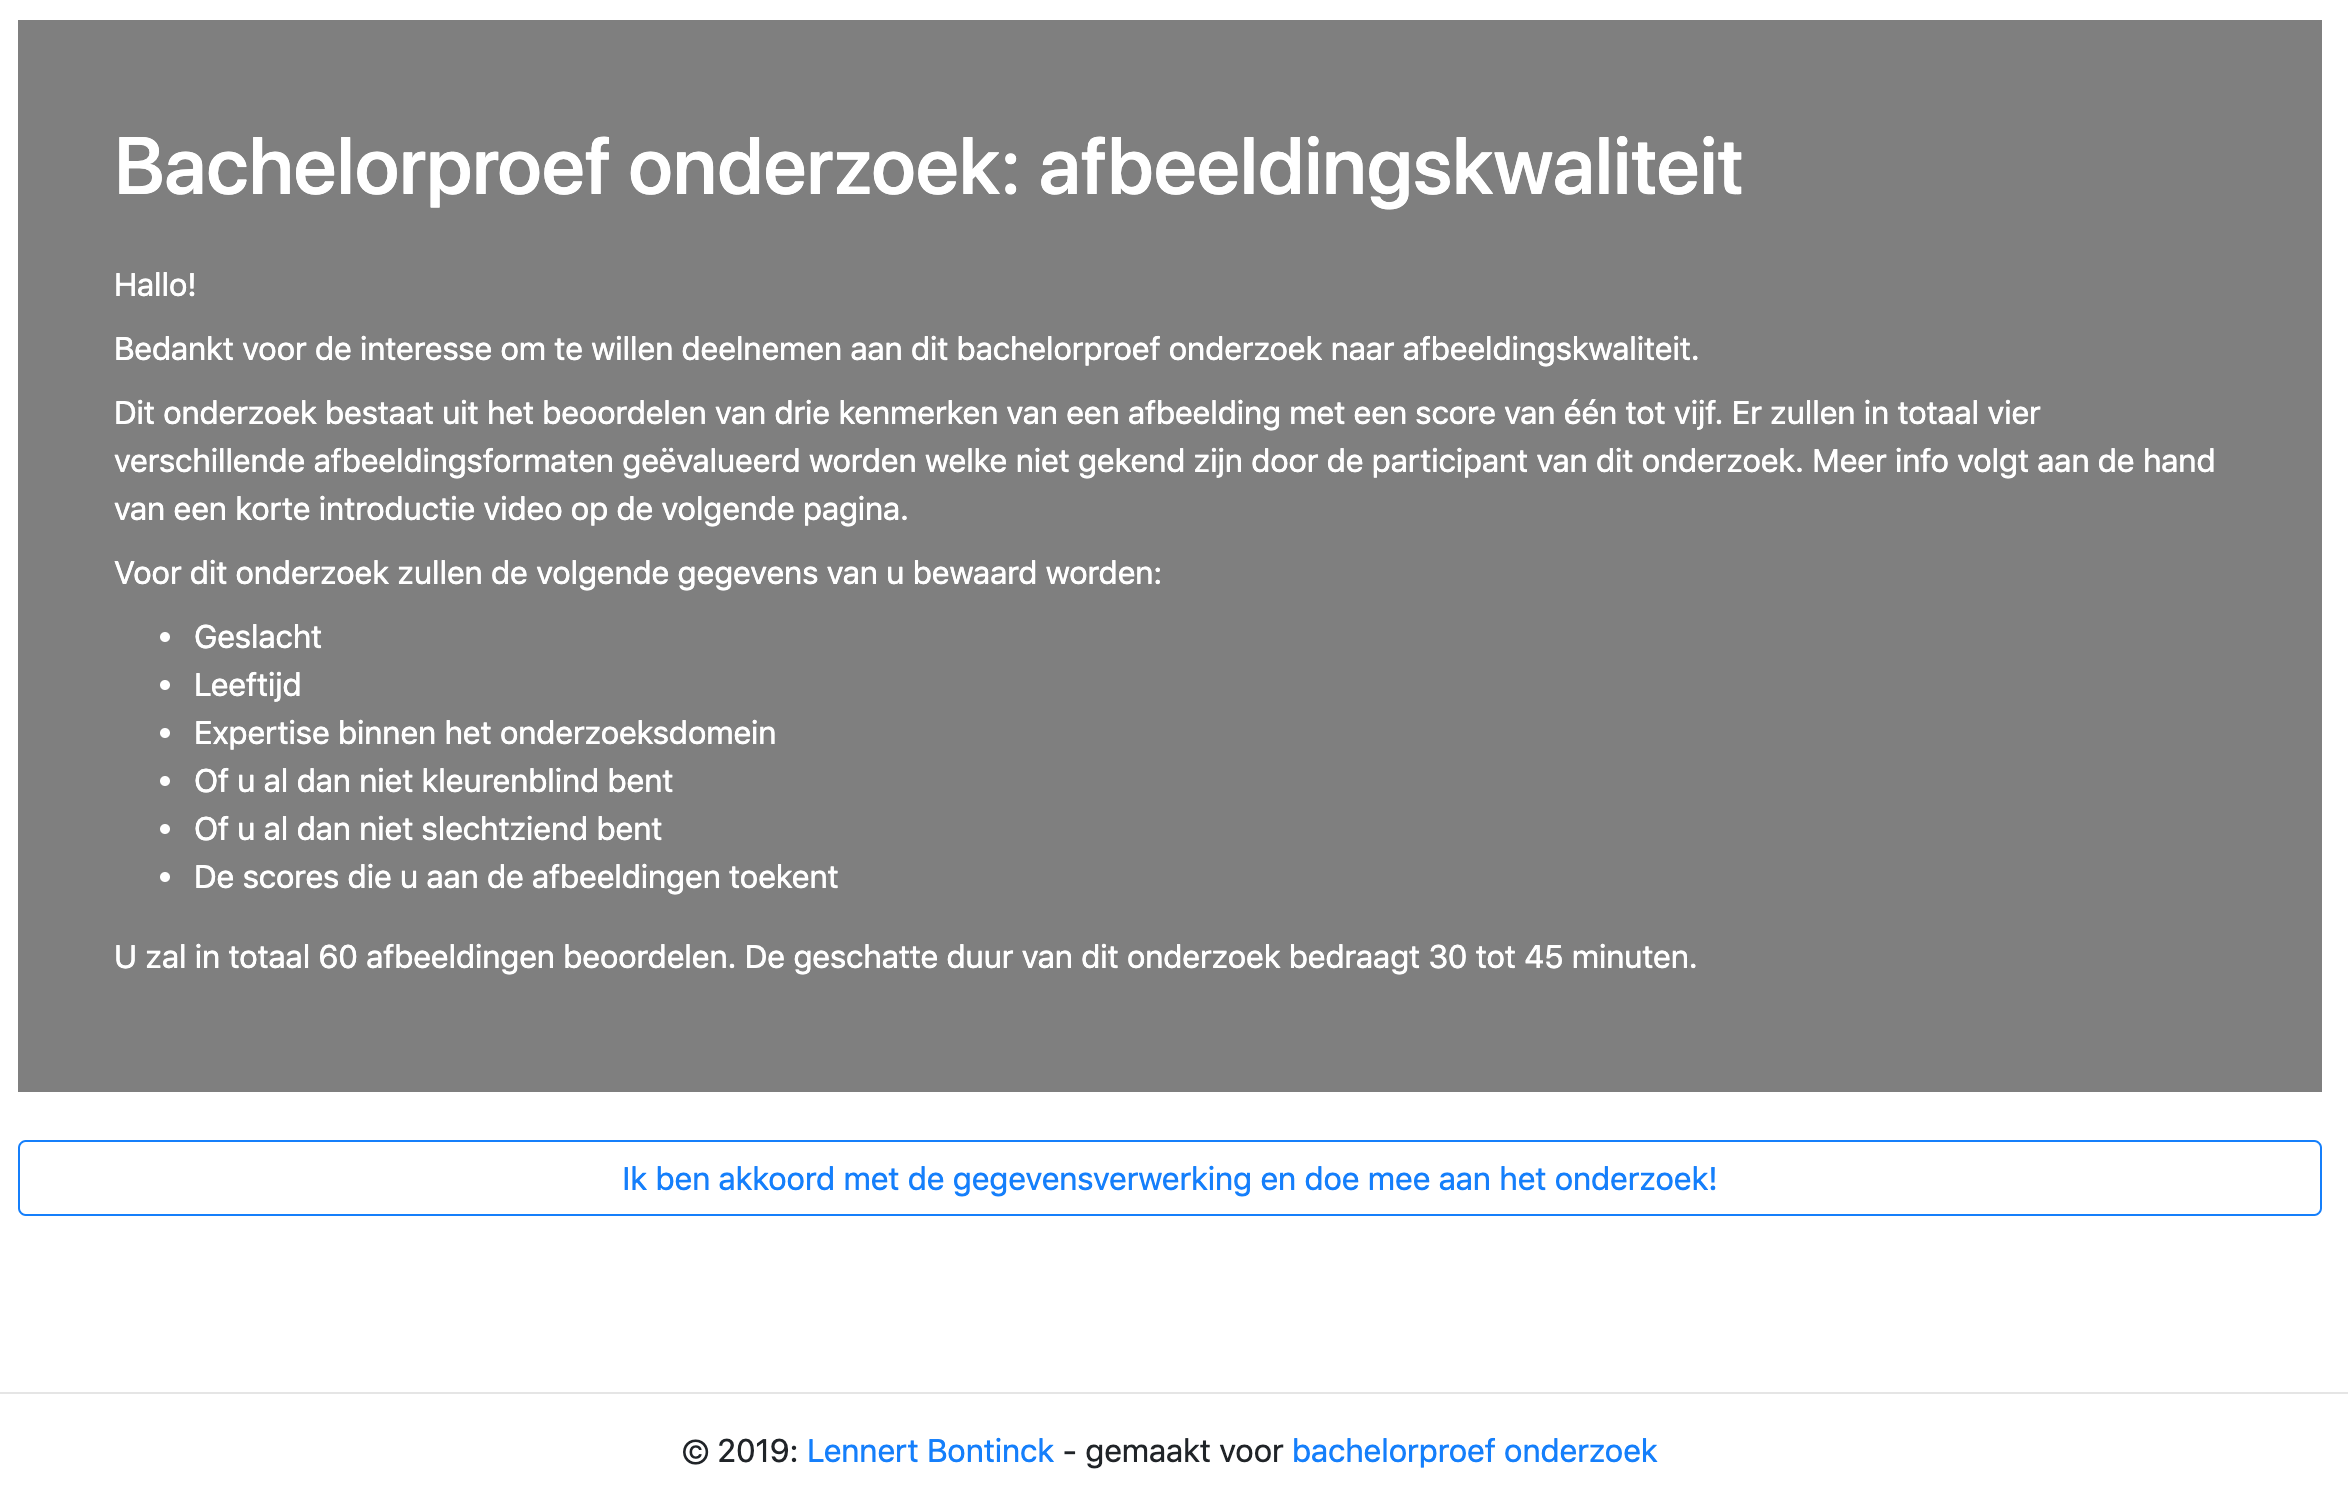
\includegraphics[width=\linewidth]{img/bijlages/afbeeldingsevaluatietool/welkom.png}
	\caption{Verwelkomingsscherm  \gls{afbeeldingsevaluatietool}}
	\label{fig:bijlages-screenshot-afbeeldingsevaluatietool-welkom}
\end{figure}

\begin{figure}	
	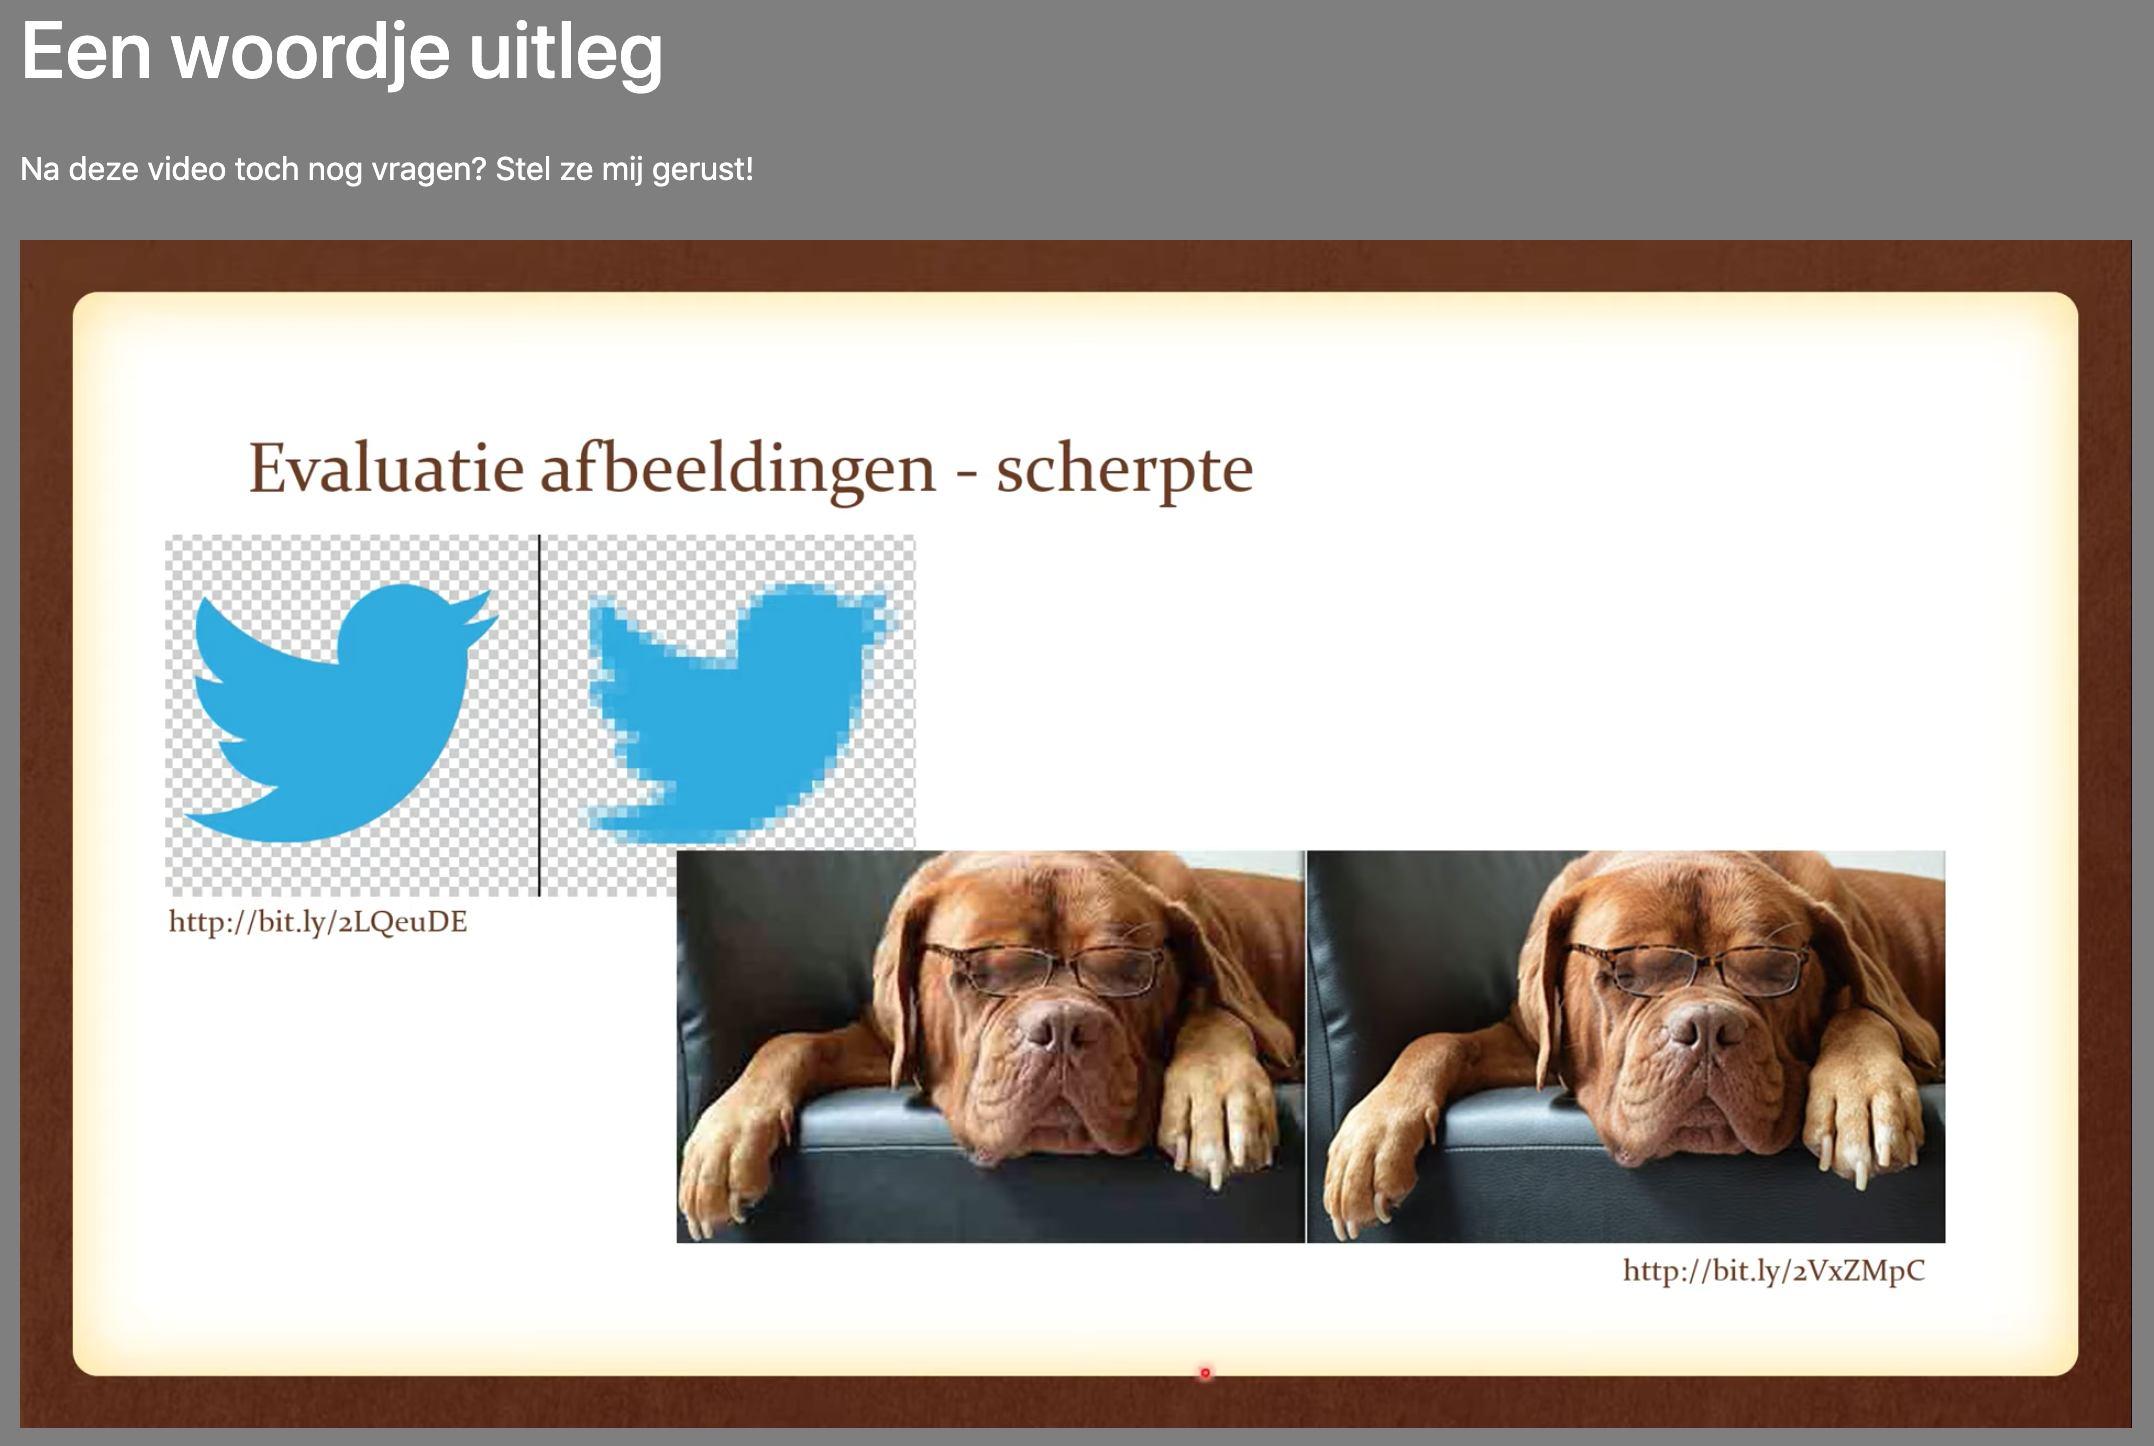
\includegraphics[width=\linewidth]{img/bijlages/afbeeldingsevaluatietool/video.png}
	\caption{Introductievideo met uitleg \gls{afbeeldingsevaluatietool}}
	\label{fig:bijlages-screenshot-afbeeldingsevaluatietool-video}
\end{figure}

\begin{figure}
	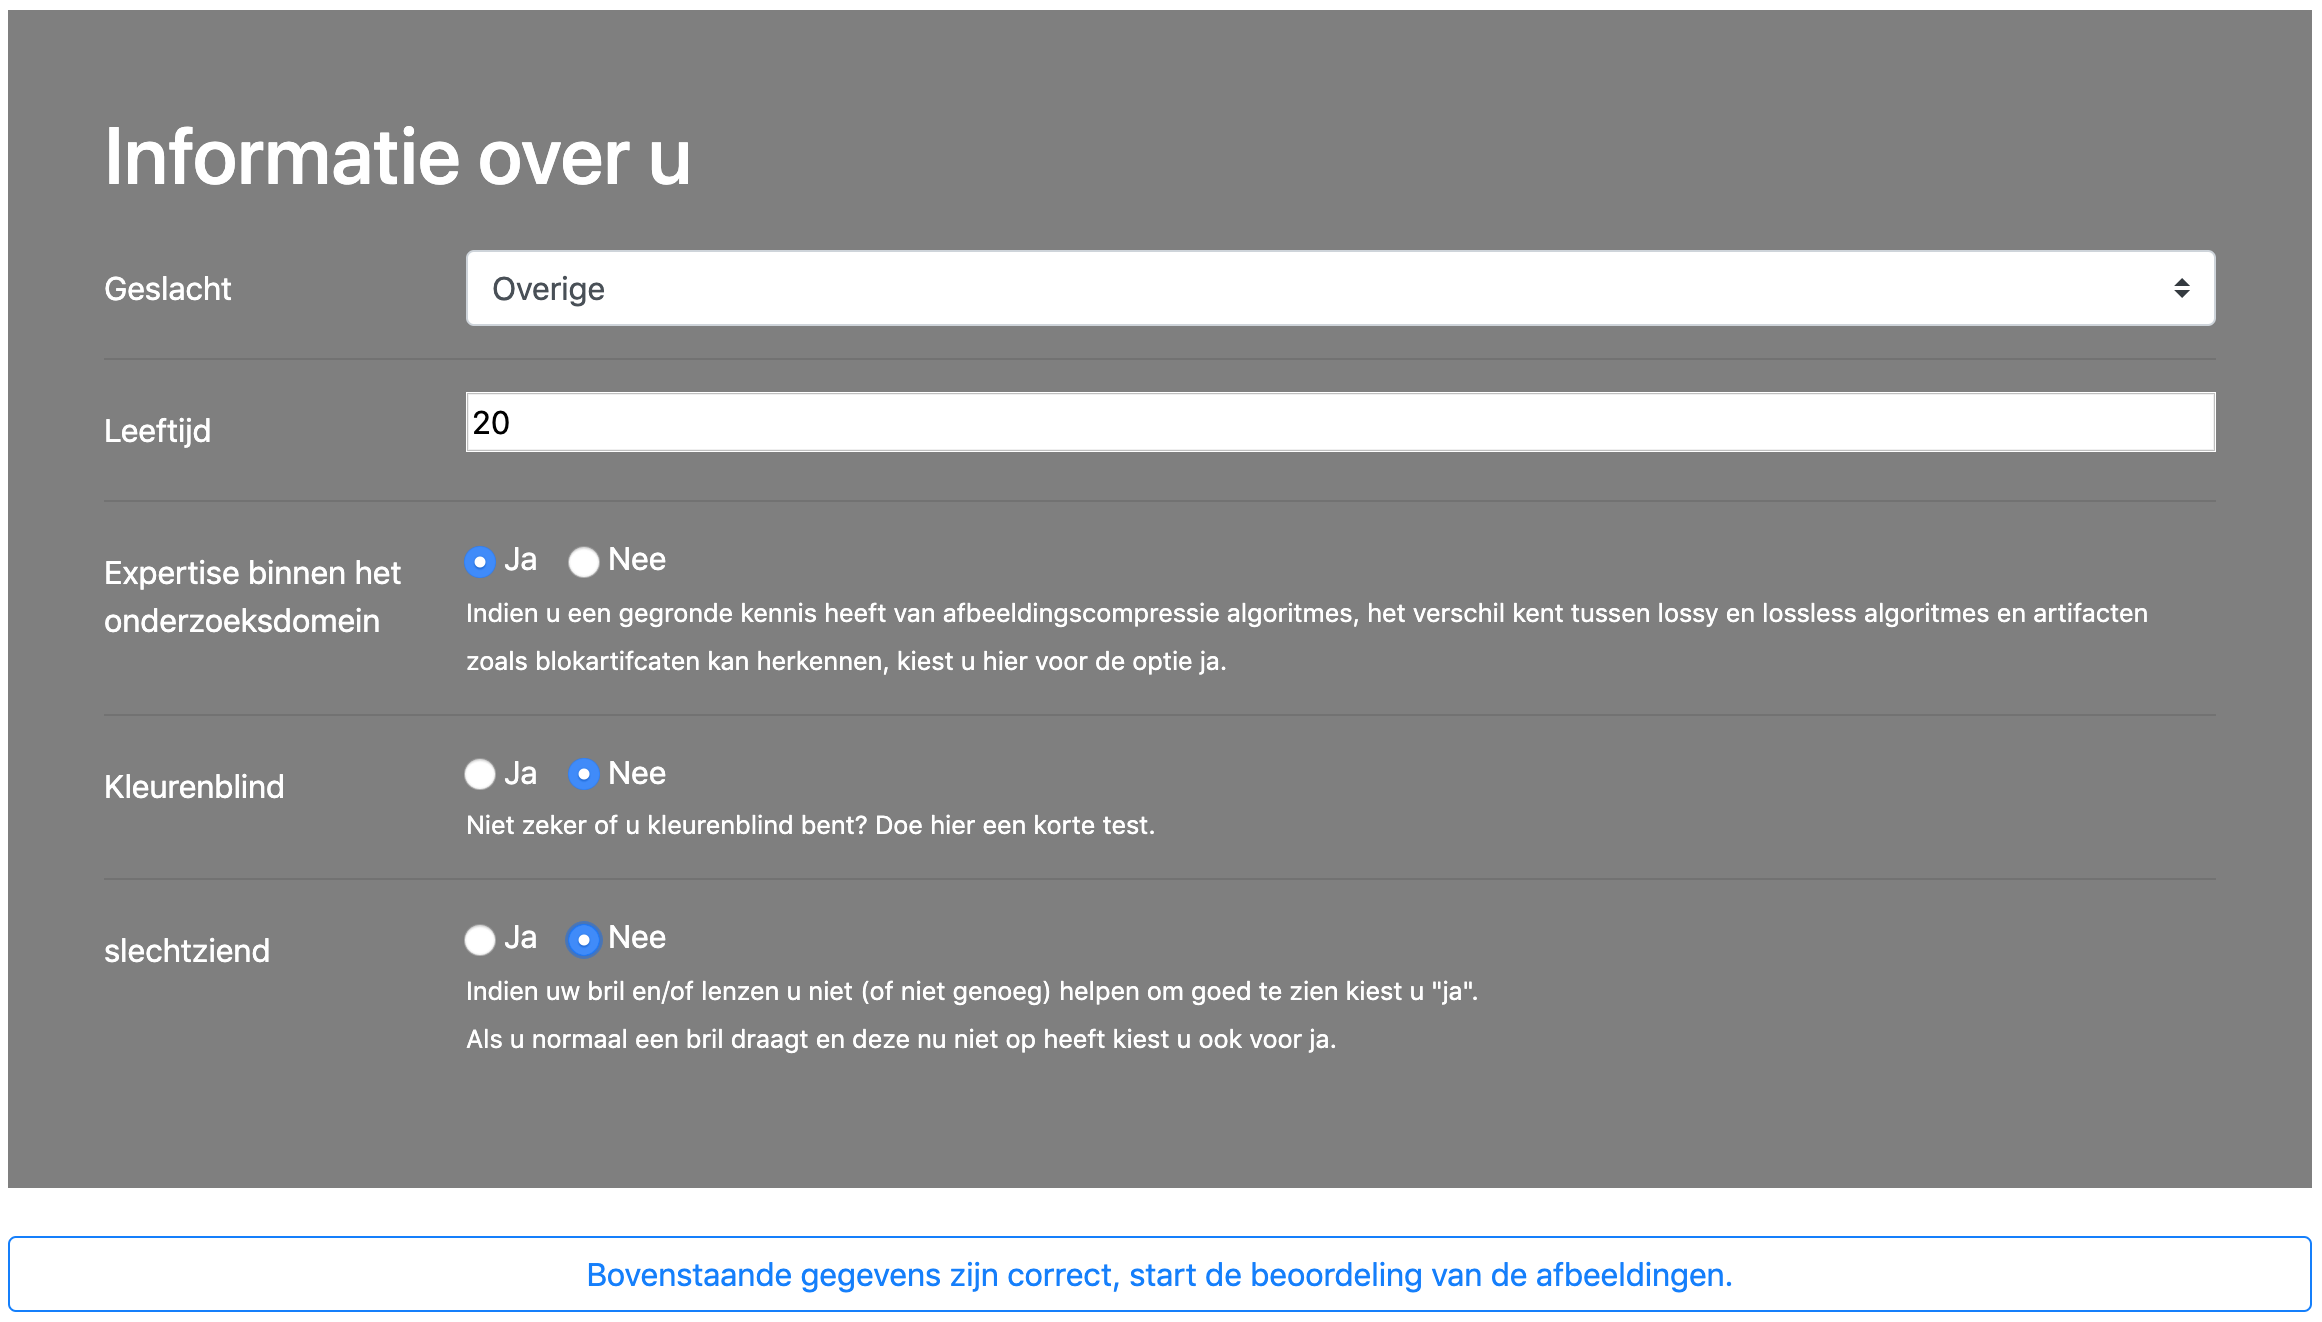
\includegraphics[width=\linewidth]{img/bijlages/afbeeldingsevaluatietool/over-u.png}
	\caption{Informatie over deelnemer  \gls{afbeeldingsevaluatietool}}
	\label{fig:bijlages-screenshot-afbeeldingsevaluatietool-over-u}
\end{figure}

\begin{figure}
	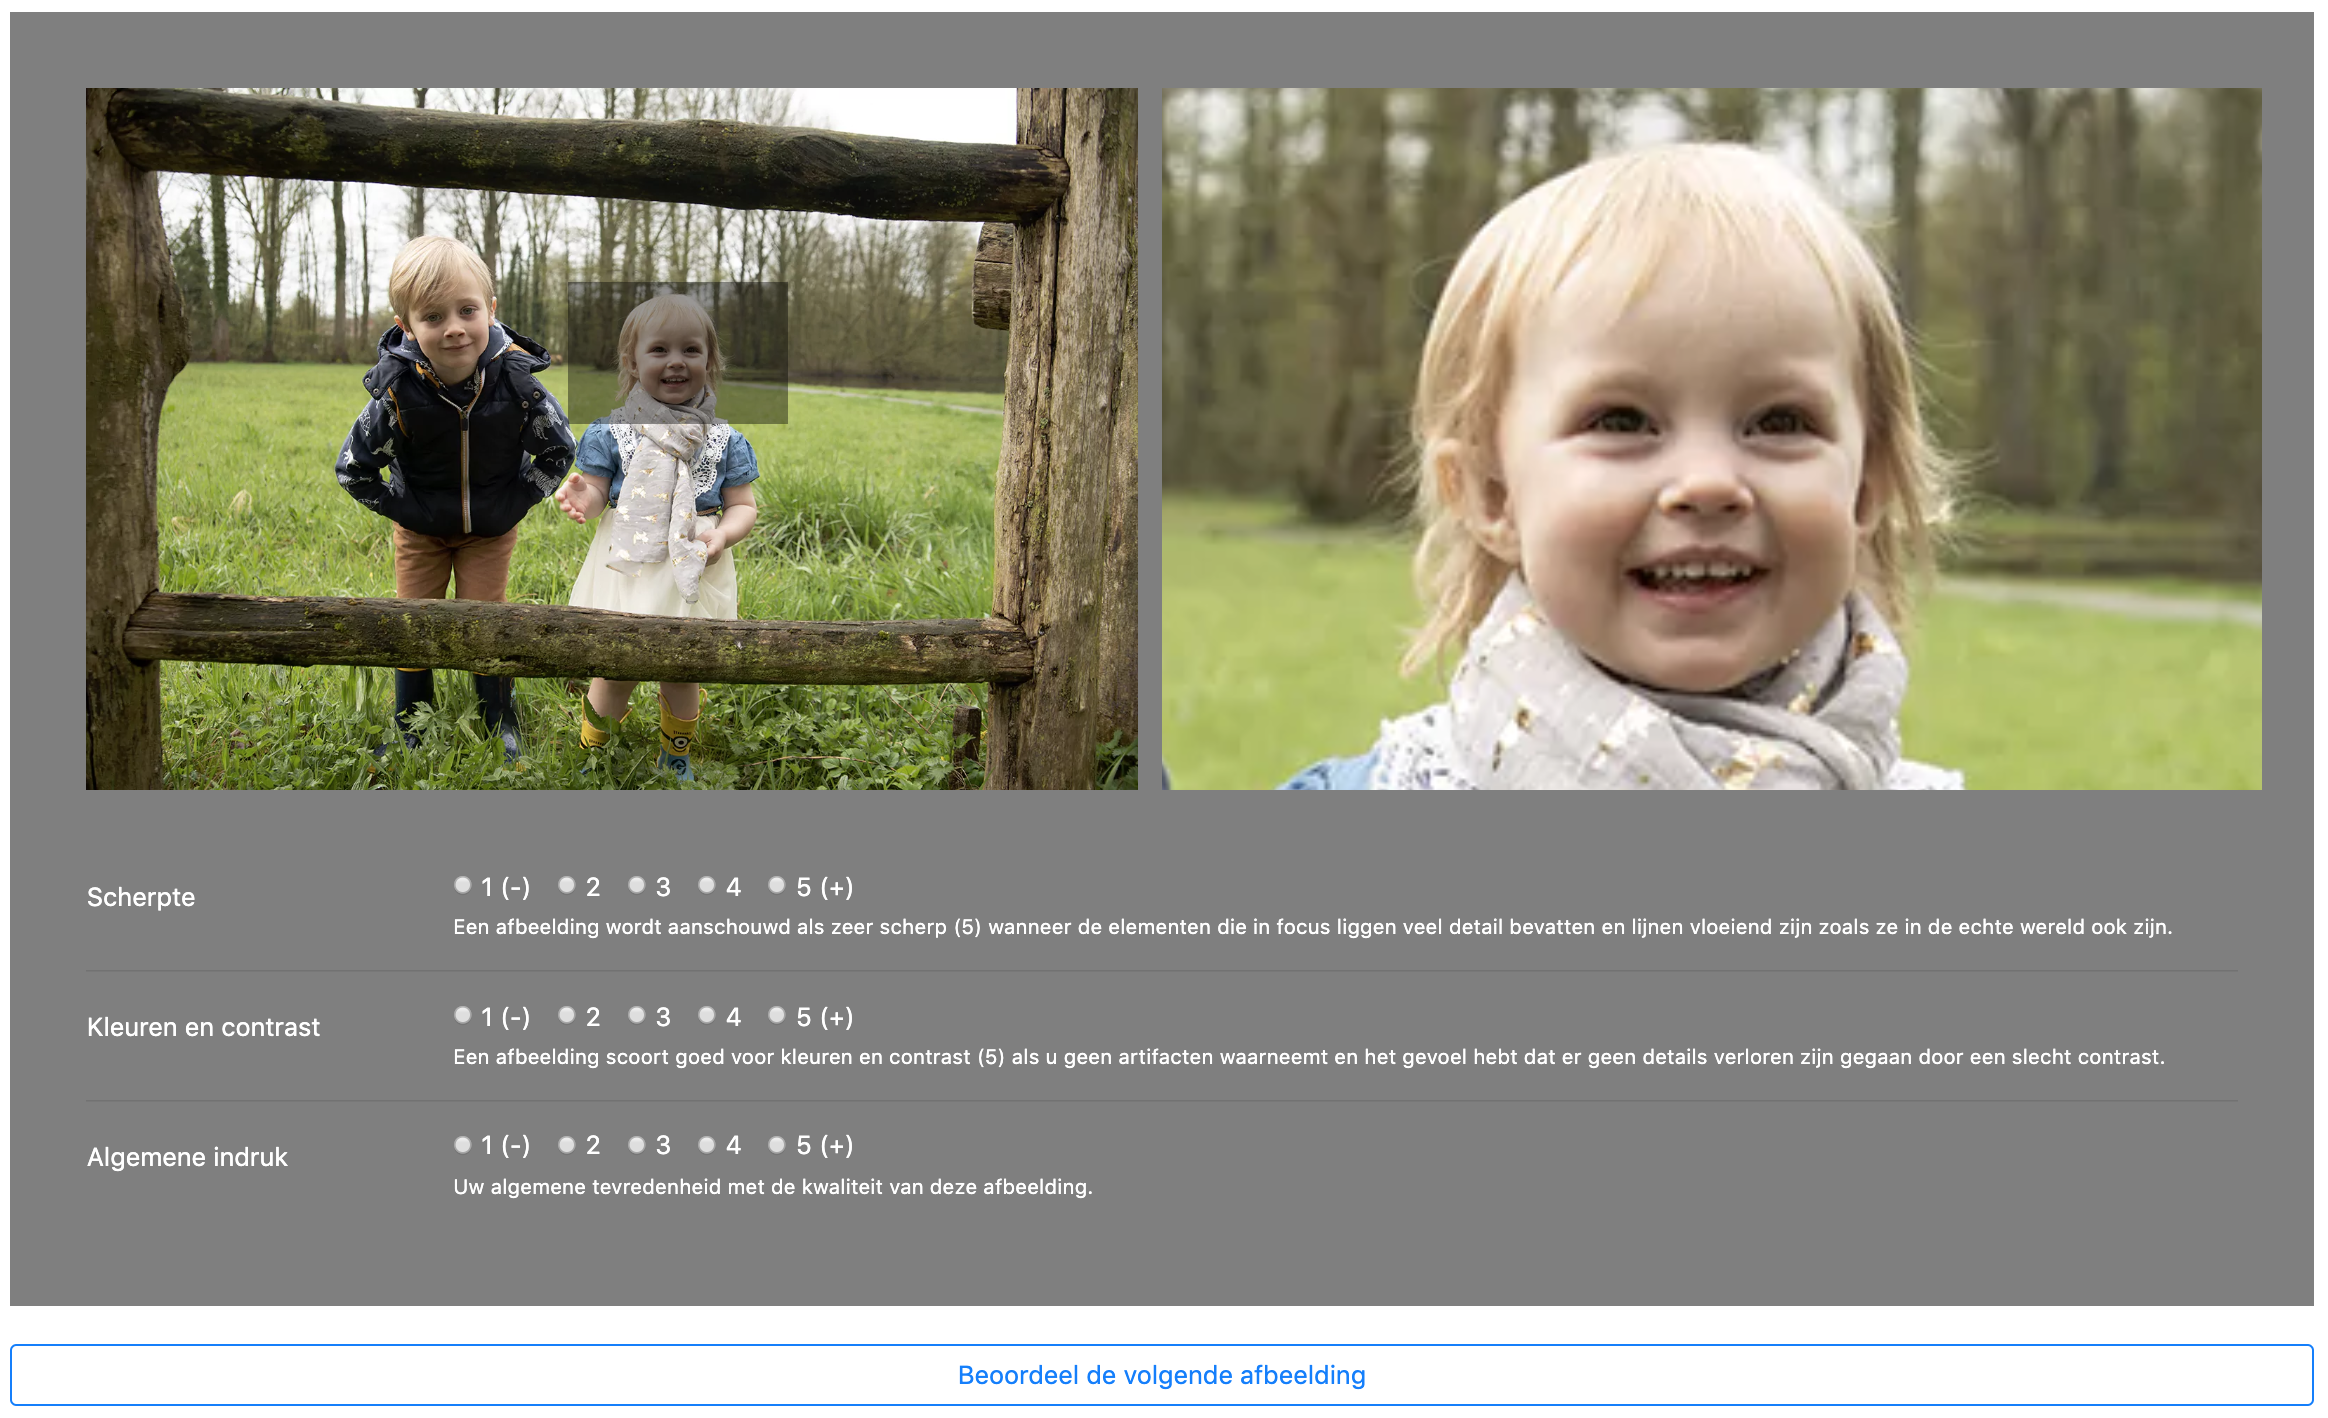
\includegraphics[width=\linewidth]{img/bijlages/afbeeldingsevaluatietool/evaluatie.png}
	\caption{Afbeelding beoordelen in de  \gls{afbeeldingsevaluatietool} met 5x zoom mogelijkheid}
	\label{fig:bijlages-screenshot-afbeeldingsevaluatietool-evalutie}
\end{figure}
